\documentclass{standalone}

\usepackage{tikz}
\newsavebox\mybox

\begin{document}
% Diagram of the TeX box model and its dimensions
% Copyright (C) 2001 by Martin Scharrer <martin@scharrer.me>, Nov 12th 2011
% This is free code under the LPPL v1.3 or later version OR the CC BY-SA 3.0
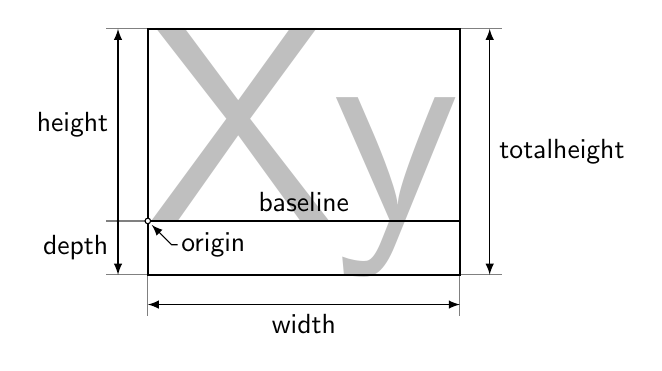
\begin{tikzpicture}[font=\sffamily,>=latex]
   % Save example text in box
   \sbox\mybox{\pgfinterruptpicture\sffamily\color{black!25}\scalebox{10}{Xy}\endpgfinterruptpicture}
   \def\HEIGHT{\ht\mybox}
   \def\WIDTH{\wd\mybox}
   \def\DEPTH{\dp\mybox}
   % Extensions lines for dimensions (drawn here to be below other material)
   \draw [gray,thin]
        (0,0)       -- +(-3.5ex,0)
        (0,\HEIGHT) -- +(-3.5ex,0)
        (0,-\DEPTH) -- +(-3.5ex,0)
        (\WIDTH,\HEIGHT) -- +(3.5ex,0)
        (\WIDTH,-\DEPTH) -- +(3.5ex,0)
        (0,-\DEPTH)      -- +(0,-3.5ex)
        (\WIDTH,-\DEPTH) -- +(0,-3.5ex)
   ;
   % Text node:
   \node [inner sep=0pt,anchor=base west] {\usebox\mybox};
   % Baseline
   \draw (0,0) -- (\WIDTH,0) node [above,midway] {baseline};
   % Box
   \draw [thick] (0,-\DEPTH) rectangle (\WIDTH,\HEIGHT);
   % Origin
   \path [fill=white,draw=black] (0,0) circle (1pt);
   \draw [<-,shorten <=2pt] (0,0) -- (2ex,-2ex) -- +(.5ex,0) node [right=-0.5ex] {origin};
   % Dimensions
   \draw [->] (-2.5ex,0) -- +(0,-\DEPTH)  node [midway,left] {depth};
   \draw [->] (-2.5ex,0) -- +(0, \HEIGHT) node [midway,left] {height};
   \draw [<->] (\WIDTH,-\DEPTH) ++(2.5ex,0) -- +(0,\DEPTH+\HEIGHT) node [midway,right] {totalheight};
   \draw [<->] (0,-\DEPTH) ++(0,-2.5ex) -- +(\WIDTH,0) node [midway,below] {width};
   \fill (-2.5ex,0) circle (.5pt);
\end{tikzpicture}
\end{document}
